\documentclass[letterpaper, 10 pt, conference]{ieeeconf}

\usepackage{graphicx}
\usepackage{amsmath,amsfonts,amssymb}

\graphicspath{ {figures/} }

\renewcommand{\vec}[1]{\boldsymbol{#1}}

\title{\textbf{AprilTrack: A Particle-Filter based AprilTag Tracker}}
\author{Daniel Pfrommer}
\date{}

\begin{document}

\maketitle

\begin{abstract}

	The AprilTrack algorithm proposed in this paper seeks to bridge two existing fields of research in computer vision literature: fiducial detection and monocular object tracking. With a rise in the popularity of fiducials, or artificial markers, as a source of ground-truth position data for mobile robots, there has been a considerable interest in designing robust and blur-resistant fiducials. Rather than devising a new fiducial, This paper attempts to improve on existing fiducials such as the popular AprilTag marker by augmenting fiducial detection algorithms with a particle-filter based monocular object tracker which reliably tracks a fiducial's position and orientation in six degrees of freedom, allowing for tag-based localization in situations where still frame based methods would be unable to do so. This novel particle-filter based algorithm is evaluated on several datasets involving both ego-motion and tag-based-motion and is compared to standalone tag detection algorithms and ground-truth tag position data.
	
\end{abstract}

\section{Introduction}


Visual tracking of fiducial markers (or simply fiducials) plays an important role in many robotics and computer vision related fields and applications, including augmented and virtual reality, visual odometry, and object tracking in 6 degrees of freedom (DOF). However, as many of these applications involve the of fiducials in structured indoors environments where illumination is often limited, long exposure times to compensate for the reduced lighting produce blurred images, especially when taken from a mobile platform such as quadrotor.


 The majority of previous literature in fiducial detection has been focused single-frame fiducial detection. A common assumption in these algorithms is that the image being processed is blur free, expectation which breaks down in empirical situations. For instance, the widely-used AprilTag [cite] marker and its successor, the AprilTag 2 [cite], rely on strong gradients between the tag's background and the surrounding white border to detect the tag. As shown in figure \ref{fig:blurred_tag}, oftentimes such algorithms fail to detect tags that have been blurred, either missing them entirely or discarding them as false positives as the identifying characteristics are completely blurred (for AprilTags this consists of a 6x6 binary grid in the center of the tag).
 
\begin{figure}[b]
	\centering
	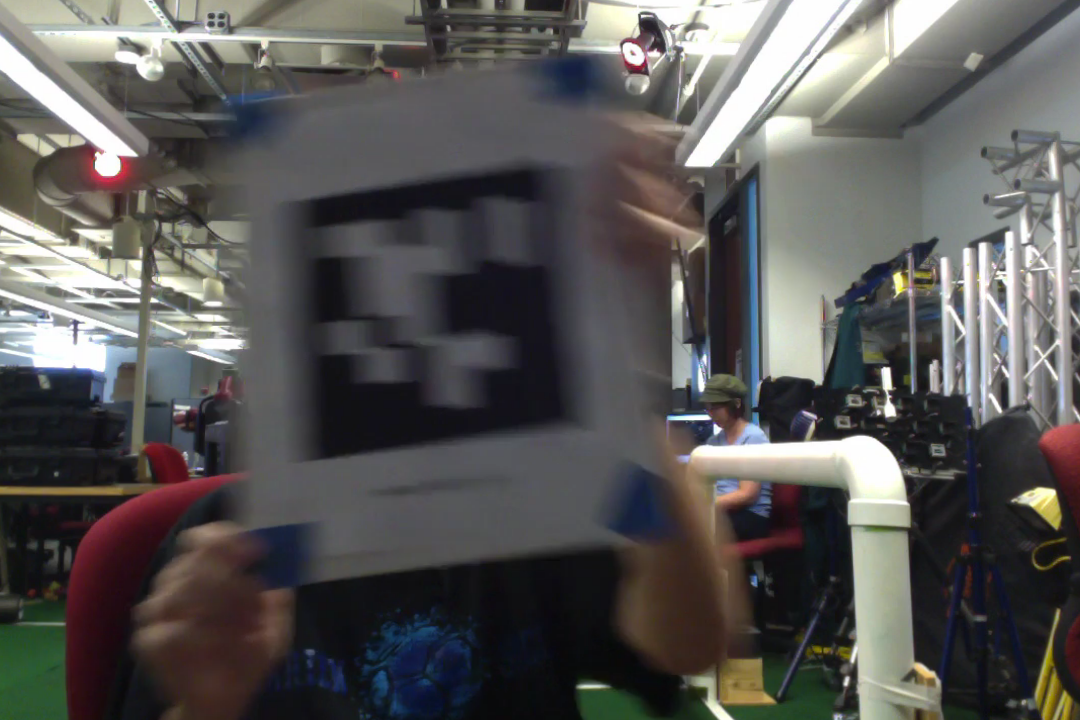
\includegraphics[width=6cm, height=4cm]{blurred_tag}
	\caption{A blurred AprilTag. Such tags are difficult for still frame based algorithms to detect as the payload (the ID encoded in the center of the tag) will cause the tag to be discarded as a false positive.}
	\label{fig:blurred_tag}
\end{figure}

There has been considerable interest in designing blur resilient fiducials. Meghshyam et al. [cite] developed ringed markers to ensure that a region of the tag will always be perpendicular to the blur direction. However, this approach, while resistent to linear blur, does not take into account more complex blurs (e.g resulting from the tag itself pivoting around an axis). In addition, the increased resilience to blur comes at the cost of localization accuracy as only the center point of the tag can be reliably determined, whereas with other tags, such as the AprilTag, full pose estimation in 6 degrees of freedom (DOF) can be done based on just a single tag.


Unlike previous attempts to engineer more resilient tags, we propose to exploit the temporal coherence between successive frames in a video sequence. As many high-blur scenarios, such as a quadroter-mounted moving camera or tracking an AprilTag-labeled moving object, involve a continuous stream of images taken at equidistant time intervals, we propose using prior knowledge on a fiducial's location to augment the detection algorithm. As such, this paper presents a novel particle-filter-based tracking algorithm (AprilTrack) capable of tracking AprilTags in 6 DOF.
	
Previous work involving the tracking of blurred objects includes the Blur-driven Tracker (BLUT) framework proposed by Wu et al. [cite] for tracking motion-blurred targets. BLUT, a particle-filter based tracker, works on the observation that blur strength can be used estimate an object's motion and provide valuable information for successfully tracking a blurred object. While capable of successfully tracking blurred objects, BLUT suffers from the disadvantage that it can do so only in two dimensions and so cannot track a sequence of motion involving arbitrary rotations and translations.


The novel method proposed in this paper is able to augment the AprilTag detector from Olson et al. [cite] with a particle-filter based tracker to successfully track an AprilTag through an arbitrary movement, providing valuable position information when existing methods would be unable to do so. In addition, the proposed algorithm is capable of incorporating the joint motion of an arbitrary number of tags to increase the accuracy of the tracked orientation.


\textbf{Overview.} The remainder of the paper is organized as follows. Section 2 gives an overview of the method proposed in this paper and describes the algorithm in detail. Section 3 describes the implementation of the algorithm and evaluates its performance on a hand-labeled dataset of blurred moving tags with both individual tag motion and multi-tag ego motion. In sections 4 and 5 we discuss the limitations of this approach and suggest possible improvements for further research.

\section{Method}

The AprilTrack algorithm is similar in concept to the BLUT tracker by Wu et al. [cite] in that it uses a particle filter to integrate all available information about a marker's position. Overall, the description of the algorithm can be broken down into 3 parts: one describing the particle filter, another on the method for evaluating candidate particles, and another describing the modifications made for tracking in multi-tag scenarios.

\subsection{The Particle Filter}

The particle filter used for the AprilTrack algorithm is a Bayesian sequential importance resampling technique which approximates a posterior distribution of state variables. There are three major steps in the algorithm: prediction, update, and resampling. We use the vector  $\vec{x}_t$  to denote the 13 dimensional state vector describing the position, orientation, velocity, and rotational velocity of the tracked target at time $t$ 

\begin{equation}
\vec{x}_t = 
\begin{bmatrix}
	\vec{r} \\
	\dot{\vec{r}} \\
	\vec{q} \\
	\vec{\omega}
\end{bmatrix}
\end{equation}

where $\vec{r}$ is the three dimensional position of the tracked object, $\dot{\vec{q}}$ is the three dimensional velocity, $\vec{q}$ is a four dimensional unit quaternion containing the pose of the tracked object, and $\vec{\omega}$ is an angular velocity with components $\omega_x$, $\omega_y$, and $\omega_z$. We use $\vec{y}_k$ to denote the measurement (appearance) of the tag a particular time $t$. 

The predicting distribution can be formulated in a Bayesian setting as the computation of the distribution $p(\vec{x}_t|\vec{z}_{t-1})$ from the prior distribution $p(\vec{x}_{t-1}|\vec{z}_{1:t-1})$:

\begin{equation} \label{eq:predict}
p(\vec{x}_t|\vec{z}_{1:t-1}) = \int p(\vec{x}_t | \vec{x}_{t-1})p(\vec{x}_t|\vec{z}_{1:t-1})d\vec{x}_{t-1}
\end{equation}

Likewise, the update step can be formulated in a similar manner, where the prior distribution is updated with the latest measurement to obtain the posterior over $\vec{x}_t$:

\begin{equation} \label{eq:update}
p(\vec{x}_t|\vec{z}_{1:t}) \propto p(\vec{z}_t|\vec{x}_t)p(\vec{x}_t|\vec{z}_{1:t-1})
\end{equation}

In this regard, particle filters attempt to approximate the posterior distribution at time $t-1$ using Monte-Carlo methods. A particle filter involves a set of $N$ samples $\{ (\vec{x}^i_{t-1}, w^i_{t-1}) \}_{i=1}^N$ where each sample is called a \emph{particle}. In the simplified case of a sequential importance resampling algorithm the prediction and update equations from \ref{eq:predict} and \ref{eq:update} can written as:

\begin{equation}
	\vec{x}^i_t \sim p(\vec{x}_t|\vec{x}^i_{t-1})
\end{equation}

\begin{equation}
	w \propto p(\vec{z}_t|\vec{x}^i_t)
\end{equation}

After selecting the particle with the highest weight as the most likely candidate, the final resampling step simply consists of drawing a new set of $N$ particles with equal weights (normalized to one) from the distribution $p(\vec{x}_t|\vec{y}_{1:t})$ where $p(\vec{x}_t|\vec{y}_{1:t})$ is approximated by the set of weighted particles.

\begin{equation}
	p(\vec{x}_t|\vec{z}_{1:t}) \approx \sum_{i=1}^{N}{w^i_t\delta_{\vec{x}^i_t}}
\end{equation}

In AprilTrack, we model $p(\vec{x}_t|\vec{x}^i_{t-1})$ as a multivariate gaussian distribution with noise $\vec{\sigma}$ around 
\begin{equation}
\vec{\mu} = 
\begin{bmatrix} 
	\vec{r}^i_{t-1} + \Delta t * \dot{\vec{r}}^i_{t-1} \\
 	\dot{\vec{r}}^i_{t-1} \\
	\vec{q}^i_{t-1} \dot{\vec{q}}^i_{t-1}\\
	\vec{\omega}^i_{t-1}
\end{bmatrix}
\end{equation}

where $\Delta t$ is the elapsed time and $\dot{\vec{q}}^i_{t-1}$ is the quaternion representation of $\Delta t * \vec{\omega}^i_{k-1}$ as described in [cite]. We also use the \emph{noise quaternion} from [cite] to apply the gaussian noise to the quaternion $\vec{q}^i_{k-1} \dot{\vec{q}}^i_{k-1}$. For simplicity, we make the assumption that the input images have been taken at equidistant time intervals and incorporate $\Delta t$ into $\vec{\sigma}$.

\subsection{Evaluation of Candidate Particles}

The successful tracking of AprilTags in 6 DOF requires a method for evaluating the likelihood of candidate particles at arbitrary three dimensional positions and rotations. To this effect, the proposed method uses homographies to generate image \emph{patches}, which are unprojected representations of an AprilTag for a particular pose and image.


Given the function $I(\begin{bmatrix} \lambda x, & \lambda y, & \lambda \end{bmatrix}^\intercal )$ representing the intensity of pixel at a particular $(x,y)$ of an image, a \emph{patch} in the image can be defined by the function 

\begin{equation}
P(x_p,y_p| \vec{H}, I ) = I(\vec{H} * \begin{bmatrix} x_p & y_p & 1\end{bmatrix}^\intercal)
\end{equation}

where $x_p$ and $y_p$ are between $-1$ and $1$ and $\vec{H}$ is a 3x3 matrix (a homography) mapping from $(x_p, y_p, 1)$ to $(\lambda x, \lambda y, \lambda)$ which incorporates the pose of an AprilTag relative to the camera. 


This allows for the evaluation of candidate particles by the measuring the similarity between the particle's patch $P^i(x_p,y_p|\vec{H}^i,I)$ in the current image and the patch from the AprilTag's last successful detection, $P_{ref}(x_p,y_p|\vec{H}_{ref},I)$. Here, $H^i$ can be calculated with

\begin{equation} \label{eq:particle_homography}
\vec{H}^i = \begin{bmatrix}
		\widehat{\vec{q}^i} & \vec{r}^i
	\end{bmatrix} \begin{bmatrix}
		\tau/2 & 0 & 0 \\
		0 & \tau/2 & 0 \\
		0 & 0 & 0 \\
		0 & 0 & 1
	\end{bmatrix}
\end{equation}



where $\widehat{\vec{q}}$ is the rotation matrix representation of particle's rotation quaternion, $\vec{r}$ is the particle's translation, and $\tau$ is the tag's edge length. The patch for the detected AprilTag uses the homography $\vec{H}_{ref}$ supplied by the AprilTag library, which computes the homography using the Direct Linear Transform algorithm [cite]. 


To compare the patches efficiently, $P^i$ and $P_{ref}$ are evaluated at a regular grid from $(-1, -1)$ to $(1, 1)$ at intervals of $2 / \rho$. This results in two $\rho \times \rho$ matrices $\vec{M}^i$ and $\vec{M}_{ref}$. To compare the patches, the error between the two  matrices is calculated using the correlation coefficient between the individual elements of the matrices.

\begin{equation}
	\epsilon(\vec{A}, \vec{B}) = \frac{1}{2} - \frac{\sum_{i=1}^{\rho} \sum_{j=1}^{\rho} (\vec{A}_{ij} - \mu_{\vec{A}})(\vec{B}_{ij} - \mu_{\vec{B}}) }{2\sigma_{A} \sigma_{B}}
\end{equation}

where $\vec{A}$ and $\vec{B}$ are the matrix approximations of two patches, $\sigma_{\vec{A}}$ and $\sigma_{\vec{B}}$ are the standard deviations of the respective matrices' elements and $\mu_{\vec{A}}$ and $\mu_{\vec{B}}$ are their means. By normalizing by mean and standard deviation, using correlation as a similarity metric (as opposed to the sum of the absolute difference or squared difference) ensures lighting invariance for comparing patches containing the same marker under different illuminations.


As in [cite] the patch error $\epsilon(\vec{M}^{i}, \vec{M}_{ref})$ is used to compute the observation likelihood $p(\vec{z}_t|\vec{x}_t)$ to update the weights and select the best particle with


\begin{equation}
	p(\vec{z}_t|\vec{x}^i_t) = exp(-\gamma \epsilon(\vec{M}^i, \vec{M}_{ref}))
\end{equation}

where the parameter $\gamma$ allows for more or less selective resampling.



\begin{figure}[b]
	\centering
	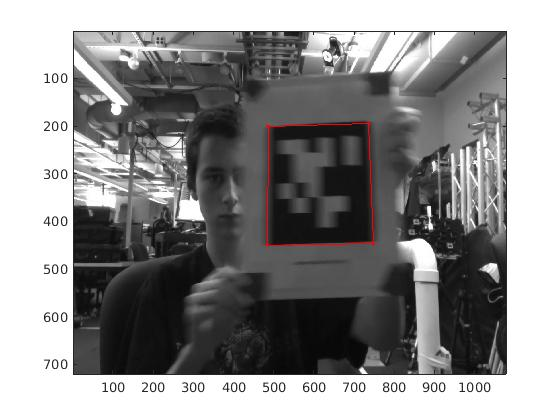
\includegraphics[width=7.5cm,height=5cm]{tracked_tag}
	\caption{A blurred tag being tracked. The red border indicates that the tag was not detected with the AprilTag detector.}
\end{figure}

\begin{figure*}[t]
	\label{fig:error}
	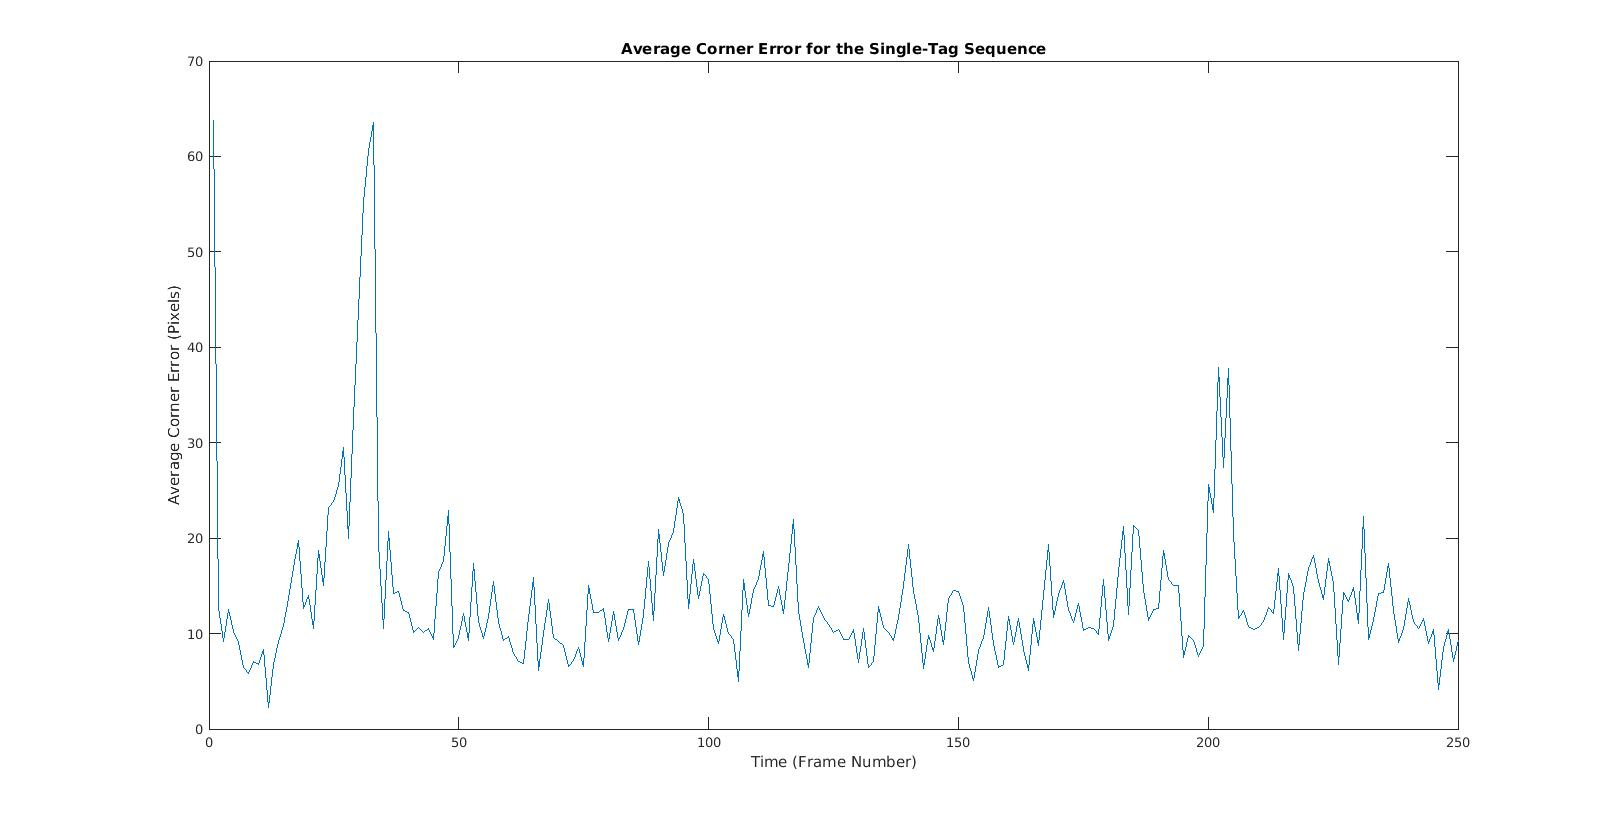
\includegraphics[width=\textwidth,height=8cm]{Average_Error}
	\caption{The average corner error between the hand-marked tag location and the tracked location. Much of the error from frames 0-200 comes from discrepancy between the tracker and the ground truth on the boundaries of blurred tags. At around frame 200, the tracker loses the tag due to a sudden rotation but is able to recover without needing a hard reset.}
\end{figure*}

\begin{figure}[b]
	\centering
	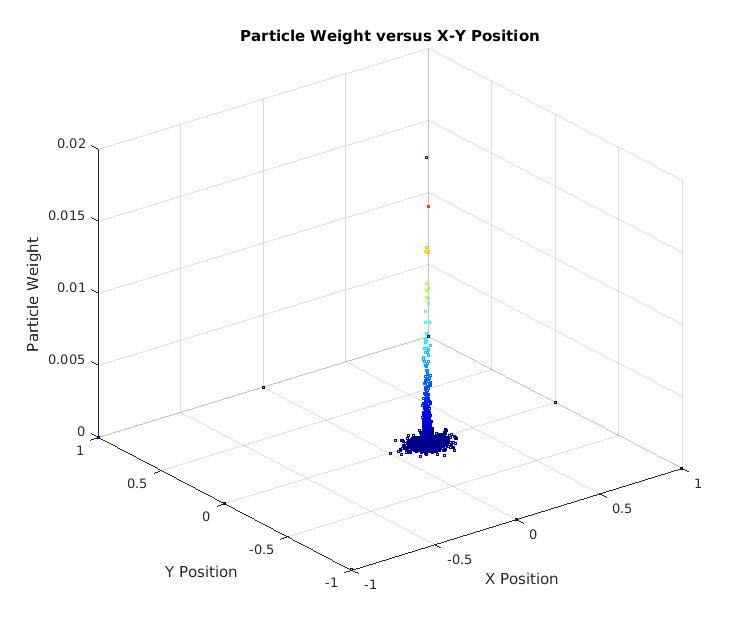
\includegraphics[width=7.5cm,height=5cm]{Particles2}
	\caption{The distribution of particles and their weights with respect to the X,Y position of the particles.}
\end{figure}

\begin{figure}[b]
	\centering
	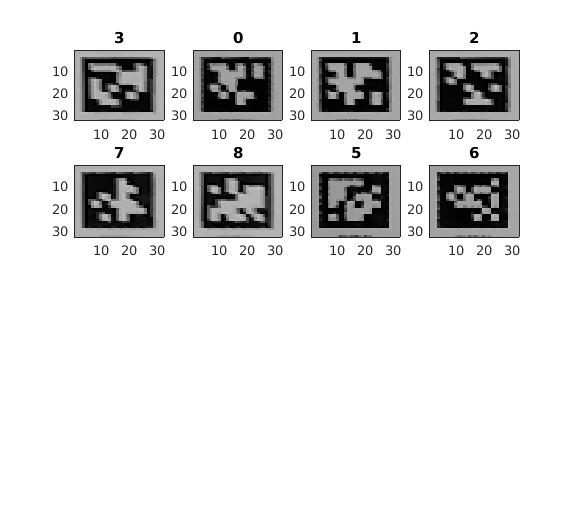
\includegraphics[width=7.5cm,height=5cm]{RefPatches}
	\caption{The reference patches of various tags (by ID) in a multi-Tag tracking scenario.}
\end{figure}

\subsection{Multi-Tag Scenarios}

To adapt this method to multi-tag scenarios, several extra parameters were introduced. In order to jointly track multiple tags, it is assumed that the relative poses of the tags are known. For each tag $T_k$ with ID $k$, the location $\vec{x}_{k}$ and orientation quaternion $\vec{g}_{k}$ are expressed such that

\begin{equation}
	\vec{X}_c = \widehat{\vec{q}^i} (\widehat{\vec{g}_k} \vec{X}_t + \vec{x}_k) + \vec{r}^i
\end{equation}
where $\vec{X}_t$ is a coordinate relative to the tag's reference frame, $\vec{X}_c$ is relative to the camera reference frame, and $\vec{q}^i$ and $\vec{r}^i$ are the position and orientation of particle $\vec{x}^i_t$. In the simple case of jointly moving tags, the $\vec{H}^i$ from equation \ref{eq:particle_homography} can then be rewritten as


\begin{equation}
	\vec{H}^i_{k} =
	\begin{bmatrix}
		\widehat{\vec{q}^i \vec{g_k}} & \widehat{\vec{q}} \vec{x_k} + \vec{r}^i
	\end{bmatrix}\begin{bmatrix}
		\tau_k/2 & 0 & 0 \\
		0 & \tau_k/2 & 0 \\
		0 & 0 & 0 \\
		0 & 0 & 1
	\end{bmatrix}
\end{equation}

where $\vec{H}^i_k$ represents the homography for particle $i$ and tag $k$ and $\tau_k$ is the edge length of tag $k$.


In the ego-motion scenario, each particle's rotation and translation can be taken to be the camera's rotation and  translation such that

\begin{equation}
	\widehat{\vec{q}^i}\vec{X}_c + \vec{r}^i = \widehat{\vec{g}_k} \vec{X}_t + \vec{x}_k
\end{equation}

resulting in the homography $\vec{H}^i_k$ and the corresponding patch approximation $\vec{M}^i_k$ where

\begin{equation}
	\vec{H}^i_k = \begin{bmatrix}
		\widehat{\vec{q}^i}^{-1} \widehat{\vec{g}_k} & \widehat{\vec{q}^i}^{-1} (\vec{x}_k - \vec{r}^i)
	\end{bmatrix} \begin{bmatrix}
		\tau_k/2 & 0 & 0 \\
		0 & \tau_k/2 & 0 \\
		0 & 0 & 0 \\
		0 & 0 & 1
	\end{bmatrix}
\end{equation}


In both ego-motion and joint tag motion, the observation likelihood $p(\vec{z}_t|\vec{x}_{t})$ then becomes

\begin{equation}
	p(\vec{z}_t|\vec{x}^i_{t}) = exp(\sum^{K}_{k=1} -\gamma \epsilon(\vec{M}^i_k, \vec{M}_{k, ref}))
\end{equation}

where $K$ is the number of tags being tracked and $\vec{M}_{k,ref}$ is the reference patch approximation for tag $k$ from the last successful detection.

\section{Results and Discussion}

The AprilTrack algorithm was primarily evluated on a manually-labeled single-tag sequence with a moving tag. The algorithm was also run on an ego-motion multi-tag sequence which will be qualitatively discussed.

\footnote{Videos of the sequences and the tracker's performance are available online at https://www.youtube.com/watch?v=BmZLKFBkcxU, https://www.youtube.com/watch?v=ebWaxO7JhKE, and }


The specific implementation of the AprilTrack algorithm used in this experiment was written in MATLAB. For both scenarios, the parameters $\gamma = 10$, $\rho=32$ were used. $\tau$ was $0.1936$ m for all tags, slightly larger than the actual tag size of $0.1635$ m to include some of the whitespace around the tag. In the single-tag scenario, the standard deviation $\vec{\sigma}$  of the gaussian noise used in the state transition distribution $p(\vec{x}_t|\vec{x}^i_{t-1})$ was $0.01$ for the $\vec{r}$ component, $0.05$ for $\vec{q}$, $0.02$ for $\dot{\vec{r}}$, and $0$ for $\omega$.


When evaluated on the single-tag sequence, the algorithm ran with $N=6000$ at around $0.5$ fps on an i7 Haswell Intel CPU. In experiments with fewer particles, it was found that the algorithm could track a tag well with as few as $1000$ particles with around $5$ fps. With a more optimized C++ implementation, the framerate could likely be brought up to $10-15$ fps, making the algorithm (run with less agressive parameters) a possible candidate for real time scenarios. Currently, the MATLAB implementation is intended for offline post-processing of a sequence.


The pixel corner error hovers at around 10 pixels for most of the sequence. The tracker loses the tag momentarily during a quick twist at around frame 200 but is able to recover rapidly without any manual intervention. Much of the error observed throughout the sequence is the result of disagreement on the boundary of a blurred tag rather than a systematic issue with the tracker itself.

When running with a multi-tag configuration, the tracker is able to make use of the additional information to more accurately track the camera's location than in a single-tag scenario. The main challenge for running the algorithm with multiple tags was not successfully tracking the tags---the algorithm was able to do that with half the particles of the single-tag scenario. Rather, the majority of the reprojection error arises from error in the relative tag positions.

\section{Conclusion}

This paper has presented the AprilTrack algorithm augmenting the standard AprilTag detection algorithm with a novel tracker capable of tracking the tags in 6 DOF by using homographies to evaluate candidate particles. Experimental results show that the tracker is capable of accurately tracking both single tags and consolidating information from multiple tags in ego-motion and joint tag-motion scenarios. In future research we plan to investigate other possible error metrics for patch comparison and look to deploy AprilTrack in realtime scenarios.


\end{document}
